\documentclass[10pt]{article}

\newcommand\code[1]{{\tt #1}}
\newcommand\smallcode[1]{{\small {\tt #1}}}
\usepackage{comment}
\usepackage{textcomp}
\usepackage{listings}
\usepackage{subfig}
\usepackage{url,wrapfig}
\usepackage{epsfig,endnotes,wrapfig}
\usepackage[aboveskip=0pt,font={small}]{caption}

\usepackage[explicit]{titlesec}
%\titleformat{\section}
 % {\normalfont\Large\bfseries}{\thesection}{1em}{#1}[{\titlerule[0.8pt]}]
\titlespacing{\section}{0pt}{*2}{*1.35}
\titlespacing{\subsection}{0pt}{*1.35}{*0.15}
%\titlespacing{\subsection}{0pt}{*1}{*0.15}
\titleformat{\subsection}[runin]{\bfseries}{\thesubsection}{1em}{#1.}[~~]
\titleformat{\subsubsection}[runin]{\slshape}{\thesubsubsection}{1em}{#1}[~~]
\titlespacing{\subsubsection}{0pt}{*0.105}{*1.00}
\titleformat{\paragraph}[runin]{\slshape}{\theparagraph}{1em}{#1}[.]
\titlespacing{\paragraph}{0pt}{*0.105}{*1.00}

\setlength{\textwidth}{6.5in}
\setlength{\oddsidemargin}{0in}
\setlength{\evensidemargin}{0in}
\setlength{\textheight}{9in}
\setlength{\topmargin}{0in}
\setlength{\headheight}{0in}
\setlength{\headsep}{0in}
\setlength{\footskip}{.5in}
\setlength{\parskip}{.05in}
\setlength{\parindent}{0in}

\begin{document}


\date{}

\title{\textbf{Design patterns for data-driven research acceleration}}

\author{Rachana Ananthakrishnan, Kyle Chard, and Ian Foster\\
The University of Chicago and Argonne National Laboratory\\
Contact: \texttt{rachana@globus.org}}

\maketitle

%Research computing centers provide high-performance storage and computing services to academic researchers. But


\flushbottom
\maketitle
\thispagestyle{empty}

\section*{Introduction}

Users of research computer centers increasingly need %more than just access to storage and computing:
%they need 
discipline-based data services.
For example, researchers may want to distribute data from a disciplinary repository, 
make data collected at a scientific instrument accessible to remote collaborators, 
allow users to upload datasets for analysis (and retrieve results), 
or accept data for publication in a public archive.
Providing such data acceleration services is a natural way for research computing centers to deliver
enhanced value to their stakeholders. 
But implementing and operating such services can be expensive and cumbersome. 

We describe here two common data-driven research acceleration design patterns 
that experience suggests are both pervasive across science and easily deployable at
research computing centers.
The purpose of a design pattern is to capture a solution to a design problem \emph{in a reusable form}~\cite{gamma1995design}.
Thus, for each design pattern we introduce the problem that it solves, describe
how it can be implemented, and present example realizations.
While these patterns can be implemented in different ways, 
our implementations  
leverage the Globus research data management platform (\url{globus.org})
to simplify development, achieve high service reliability, and reduce administrative overheads associated with the operation of sophisticated services. 
 
%We describe how each pattern can be implemented easily and reliably by combining research computing center
%facilities with services provided by the Globus research data management platform,
%and present examples of their use.
%
%We describe here a set of data management use cases that are representative of needs across a range of scientific domains and institutions that use these design patterns, thus enhancing the value of existing research computing center infrastructure. 
%In each case we outline how the use of the Globus platform simplifies development, improves service reliability, and reduces administrative overheads needed to support complex services. 

%We introduce here two design patterns relevant to data-intensive science at research computing centers.
%For the first, we point to an online reference implementation and associated article that describes in considerable detail how to realize this design pattern in different environments.
%The second is described in less detail, although several open source implementations 

\section*{Design pattern \#1: The Modern Research Data Portal}

This first pattern addresses the need for high performance and secure delivery of 
large amounts of data.  
The need for exchange data has led to an explosion over recent decades in the
number and variety of \textbf{research data portals}:
systems that provide remote access to data repositories for 
such purposes as discovery and distribution of reference data,
data upload for analysis and/or integration, 
and data sharing for collaborative analysis.
In most such systems, a web server reads and writes a directly connected data repository 
in response to client requests.

The relative simplicity of this structure has allowed it to persist largely unchanged from the 
first days of the web.
However, its monolithic architecture---in particular, its tight integration of 
control channel processing (request processing, user authentication) and 
data channel processing (routing of data to/from remote sources and data repositories)
has increasingly become an obstacle to performance, usability, and security.

The \textbf{modern research data portal} (MRDP) design pattern~\cite{BMRDP}
re-imagines the data portal in a much more scalable and performant form.
As illustrated in Figure~\ref{fig:simple},
portal functionality is decomposed along two distinct but complementary dimensions.
First, control channel communications and data channel communications are separated,
with the former handled by a \textbf{portal web server} computer deployed (most often) in the institution's enterprise network
and the latter by specialized \textbf{data servers} connected directly to high-speed networks
and storage systems in a Science DMZ~\cite{dart2014science}.
Second, responsibility for managing data transfers, data access, and sometimes also authentication is
outsourced (in our examples, to cloud-hosted \textbf{Globus services}).
The design pattern thus defines distinct roles for the portal server, 
which manages who is allowed to do what;
data servers, where authorized operations are performed on data;
and Globus services, which orchestrate data access. 

The portal server is at the heart of the MRDP implementation. 
It sits behind the institutional firewall, from where it serves up web pages to users, 
responds to HTTP requests, 
and issues REST communications to Globus services (and optionally other services) to implement MRDP behaviors. 
The REST communications are central to the power of the MRDP design pattern, 
as it is they that let the web server outsource many of the complex tasks associated with portal operations. 
Only the web server component needs to be provided for a specific implementation.


\begin{wrapfigure}[21]{r}{3.2in}
\vspace{-6ex}
    \centering
    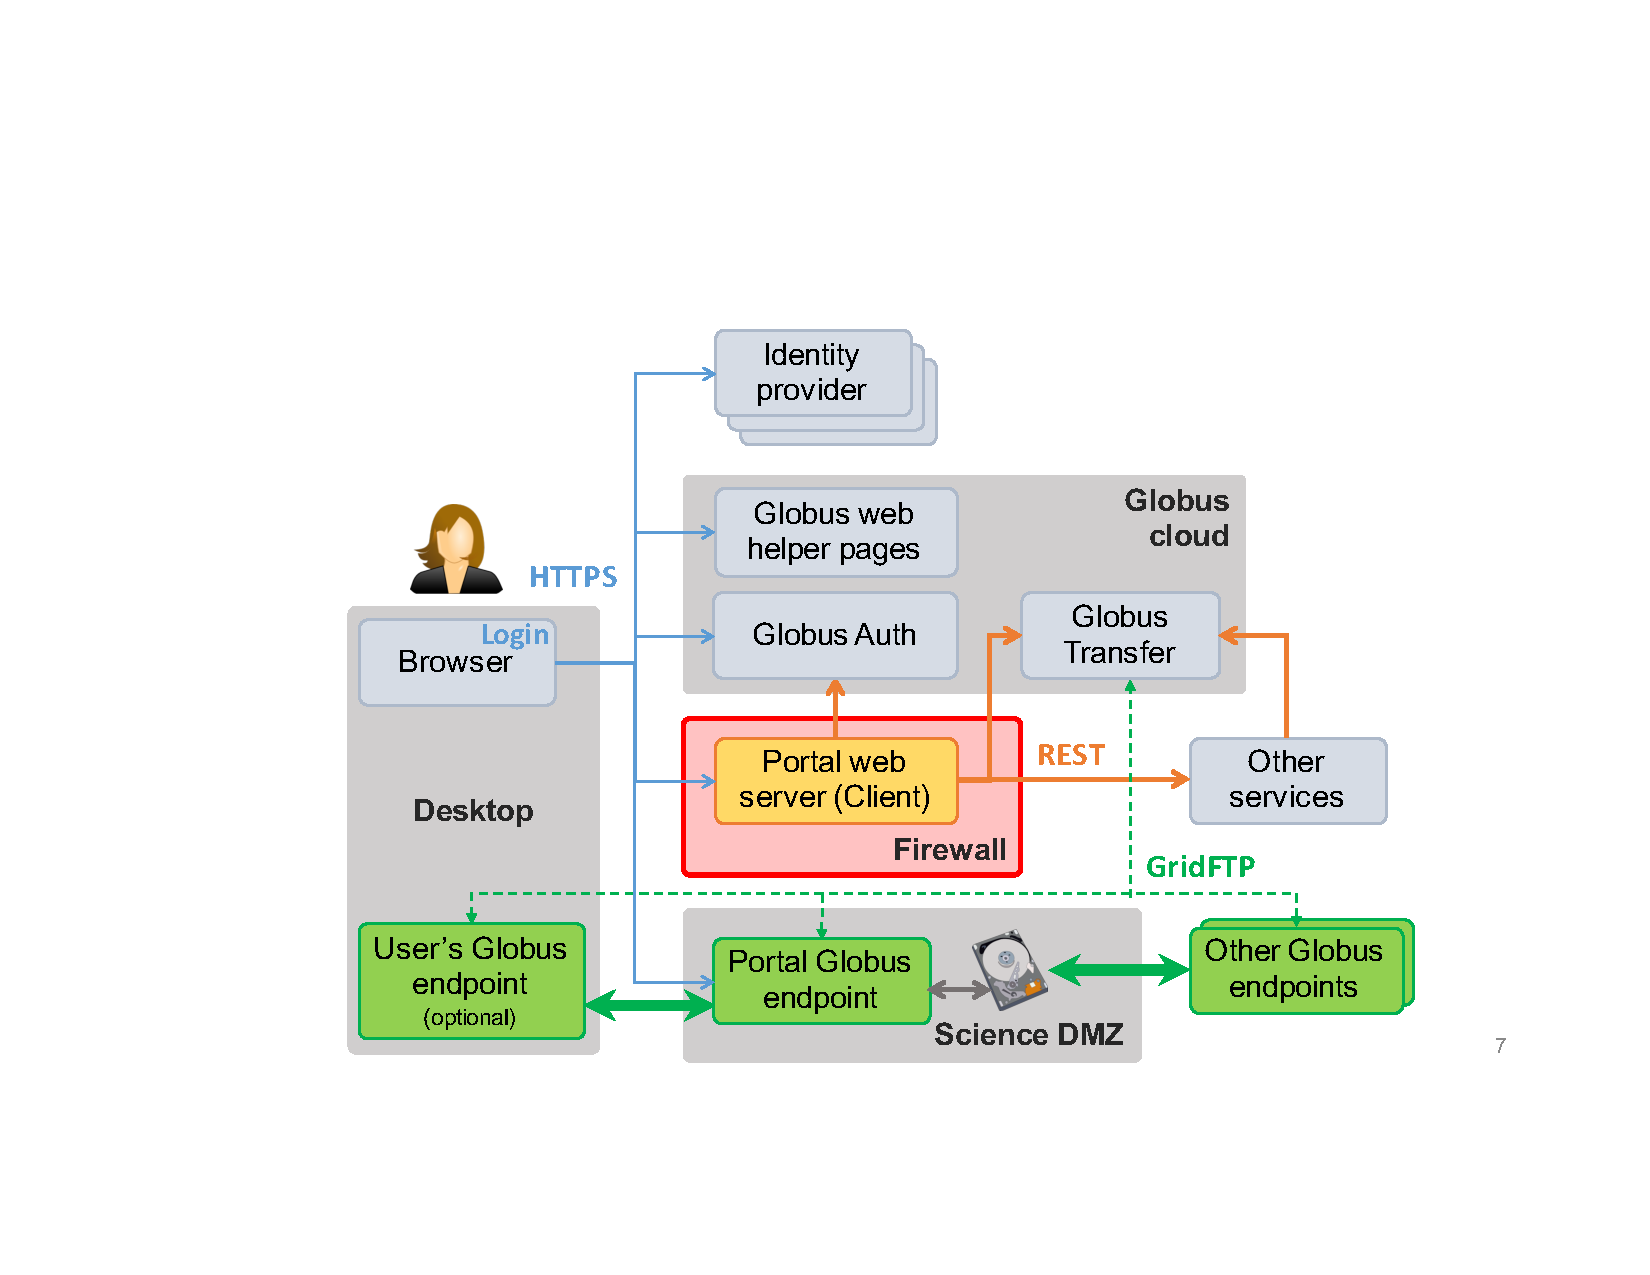
\includegraphics[trim=2.3in 1.2in 1.5in 2.1in,clip,width=0.5\columnwidth]{Figures/ResearchDataPortal-new.pdf}
    \caption{MRDP basics. Clients (left) authenticate with 
    %any one of many identity providers 
    an identity provider (top) and connect to the portal web server (center) that implements the domain-specific portal logic.
    The portal web server, sitting behind the institutional firewall (red),
    %responds to client requests by using 
    uses REST APIs
    to direct Globus cloud services (top) to operate on data in the Science DMZ (bottom center) and/or to interact with other services (center right).
    Data flows reliably and securely between Globus endpoints without traversing the firewall.
    \label{fig:simple}}
\end{wrapfigure}

A separate document provides a detailed description of the MRDP design pattern~\cite{BMRDP}
and a companion web site, \url{docs.globus.org/mrdp}, provides a reference implementation that the reader can deploy
and adapt to build their own MRDP.

The basic MRDP design pattern is concerned with enabling high-speed download of data hosted
on research computing center storage.
Many variants of this basic pattern have been constructed.
For example, the data that users access may come from an experimental facility rather than a data archive, 
in which case they may be deleted after download. 
Access may be granted to groups of users rather than individuals.
Data may be publicly available; alternatively, access may require approval from portal administrators.
A portal may allow its users to upload datasets for analysis and then retrieve analysis results.
A data publication portal may accept data submissions from users, 
and load data that pass quality control procedures or curator approval into a public archive.
Each of these variants can naturally be expressed in terms of the MRDP design pattern.

%The scientific process is based on the need to share, extend, and validate results. 
%In the world of data-driven discovery, there is a need to share not only final published data, but also raw and intermediary data. 
%While data portals have long been used for this purpose, they have several significant shortcomings: they are not readily equipped to take advantage of high performance data transfer infrastructure; 
%they do not provide methods to ensure data reliability; 
%and they are developed from scratch, with each ad hoc deployment implementing its own authentication, authorization, and data transfer functionality. 
%When dealing with few users and small amounts of data, these problems are not prohibitive, 
%but as data sizes grow, the legacy research data portal is unable to address user needs. 

%The modern research data portal is based upon the maturation of two independent efforts aimed at decoupling research data access from enterprise networks, on the one hand, and research data management logic from storage system access, on the other. 
%These developments inspired a new approach to the construction of research data portals based on a decomposition of the previously monolithic data portal architecture into three distinct components: 
%
%\begin{enumerate}
%\item
%The portal server (a web server) which handles data search and access, mapping between users and datasets, and other web services tasks;
%\item
%A high-performance network enclave that connects large-scale data servers directly to high-performance networks (e.g., the Science DMZ); and
%\item
%a reliable, high-performance external data management service with authentication and other primitives based on standard web APIs (e.g., Globus).
%\end{enumerate}


%The data channel is completely separated from the control channel. That is, all data sits external to the portal server. Globus Connect servers are deployed next to storage systems enable high-speed, reliable, and secure access to those storage systems. They may be
%deployed within a Science DMZ, on a user's personal computer, on a cloud system, or elsewhere. Each endpoint implements the GridFTP protocol for high-speed endpoint-to-endpoint data transfer and the HTTPS protocol  to enable access to endpoint storage from a web client.  
%For high performance data access, the Globus endpoints are deployed on high performance data transfer nodes (DTNs) that sit within a Science DMZ.
%
%The MRDP uses external services, such as Globus, to manage authentication and authorization as well as secure data access. 

\subsection*{MRDP case study: Data distribution at the ARM Climate Research Facility} 

The Atmospheric Radiation Measurement (ARM) Climate Research Facility data archive, hosted at Oak Ridge National Laboratory, makes available continuous measurements data from field campaigns. 
The archive adds about about 20 TB of data per month, 
and provides both data products and value added products. 
Increasing data volumes per user request makes simple in-browser download options insufficient, and scalable and reliable data transfer mechanisms are needed for end users. 
The facility also recognizes that results from user data requests need to be made available only to those users, and protected from access by others. 

\begin{wrapfigure}[16]{r}{4in}

    \vspace{-2ex}

    \centering
    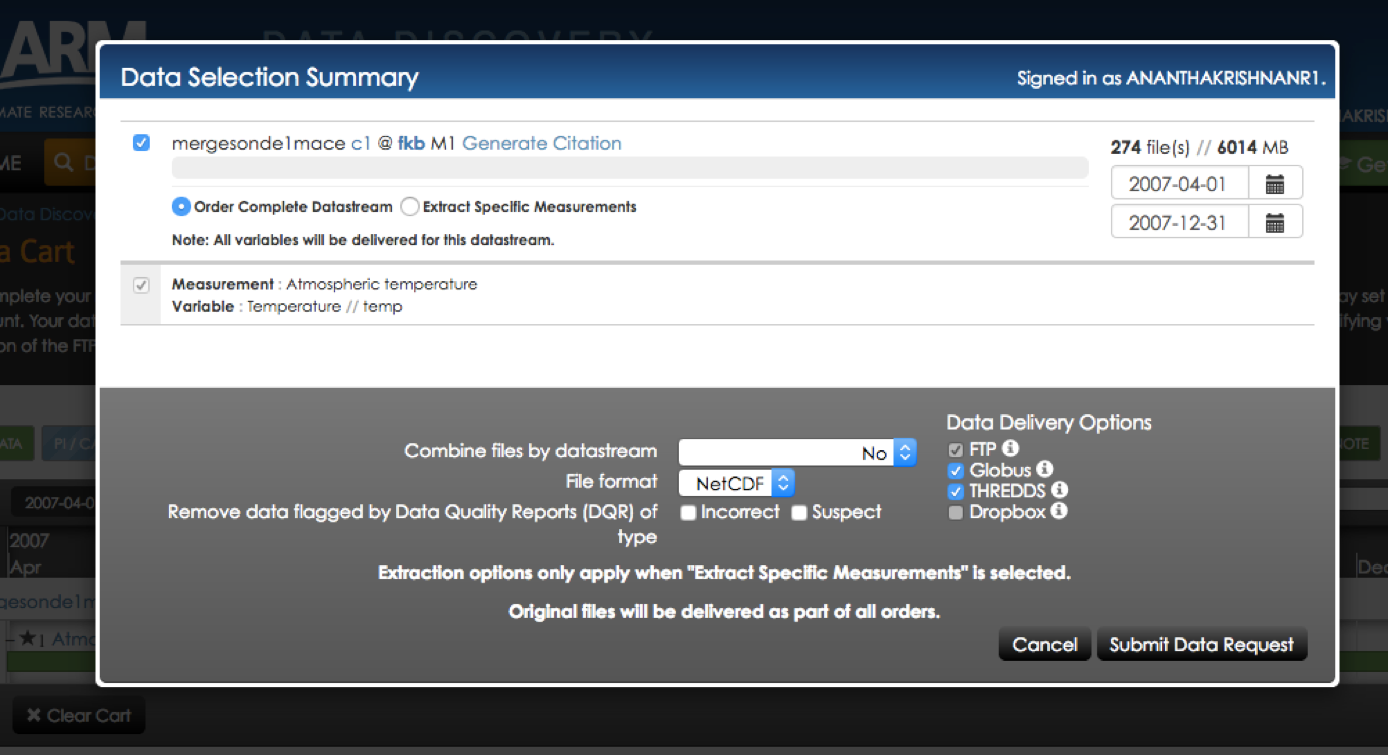
\includegraphics[trim=0.63in 0.45in 0.31in 0.26in,clip,width=0.62\columnwidth]{Figures/ARM.png}
    
    \vspace{1ex}
    
    \caption{A snapshot of the ARM data selection and download interface, 
    showing the Globus option selected at middle right. 
    \label{fig:ARM}}
\end{wrapfigure}

To address these challenges, ARM uses Globus platform APIs to integrate support for the Globus data sharing solution with their data processing system. 
Specifically, they use the APIs to create folders for each data request and to configure permissions such that only users who need access to the data can access the folder. 
A link to the shared folder is included in the notifications the ARM platform sends to its users when the data product is ready for download. 
With data access via the DTN node setup at ORNL, and Globus monitoring tools providing insights into transfer activities, the ARM team can provide their users a highly scalable and managed solution for data access. 
This use of the Globus platform APIs allows ARM  to offer their familiar interfaces and portal to their users, with minimal change in their workflow to access enhanced data access tools.



\subsection*{MRDP case study: NCAR Research Data Archive}

The Research Data Archive (RDA) project at the National Center for Atmospheric Research (NCAR) has a repository of several petabytes of climate data that they make available to the community. In addition to providing interfaces for data access, RDA also allows users to request derived or processed data, such as the results of re-analysis and subsetting operations. The primary interface for RDA users is a data portal that has search, download and processing capabilities. 

With growing data volumes, the RDA team identified the need for a scalable data management solution that included efficient and managed data transfer for end users. 
Leveraging the MRDP pattern, they integrated Globus sharing and transfer solutions to serve data to their users. 
RDA users continue to use their RDA login, search and discover datasets of interest, and optionally request derived data from the RDA portal. 
The RDA portal processes the request, and places the data on a Globus shared endpoint on a DTN hosted and operated at NCAR. 
The DTN is hosted on their Science DMZ, decoupled from the RDA portal, and configured and tuned for efficient data transfer. 
Using Globus APIs to integrate this into their data distribution workflow, RDA manages permissions on the shared endpoint to ensure the processed data is available only to the user who requested it. The user is notified once the data is ready for transfer via Globus. With the RDA login integrated with Globus Auth, the users get single sign on across the portal and Globus for data access and transfer. 

The RDA services also monitor the data transfer activity to identify any issue and help in debugging them, and to determine if the user has downloaded the data made available. 
Figure~\ref{fig:sizetime}, from Chard et al.~\cite{BMRDP}, show the diversity of data downloads
performed by a working MRDP instance, and (on the right), the high performance that can be
achieved when both source and destination operate appropriately configured DTNs. 

  \begin{figure}[t]
  \centering
  \subfloat[RDA]{\label{fig:rda-rate}
  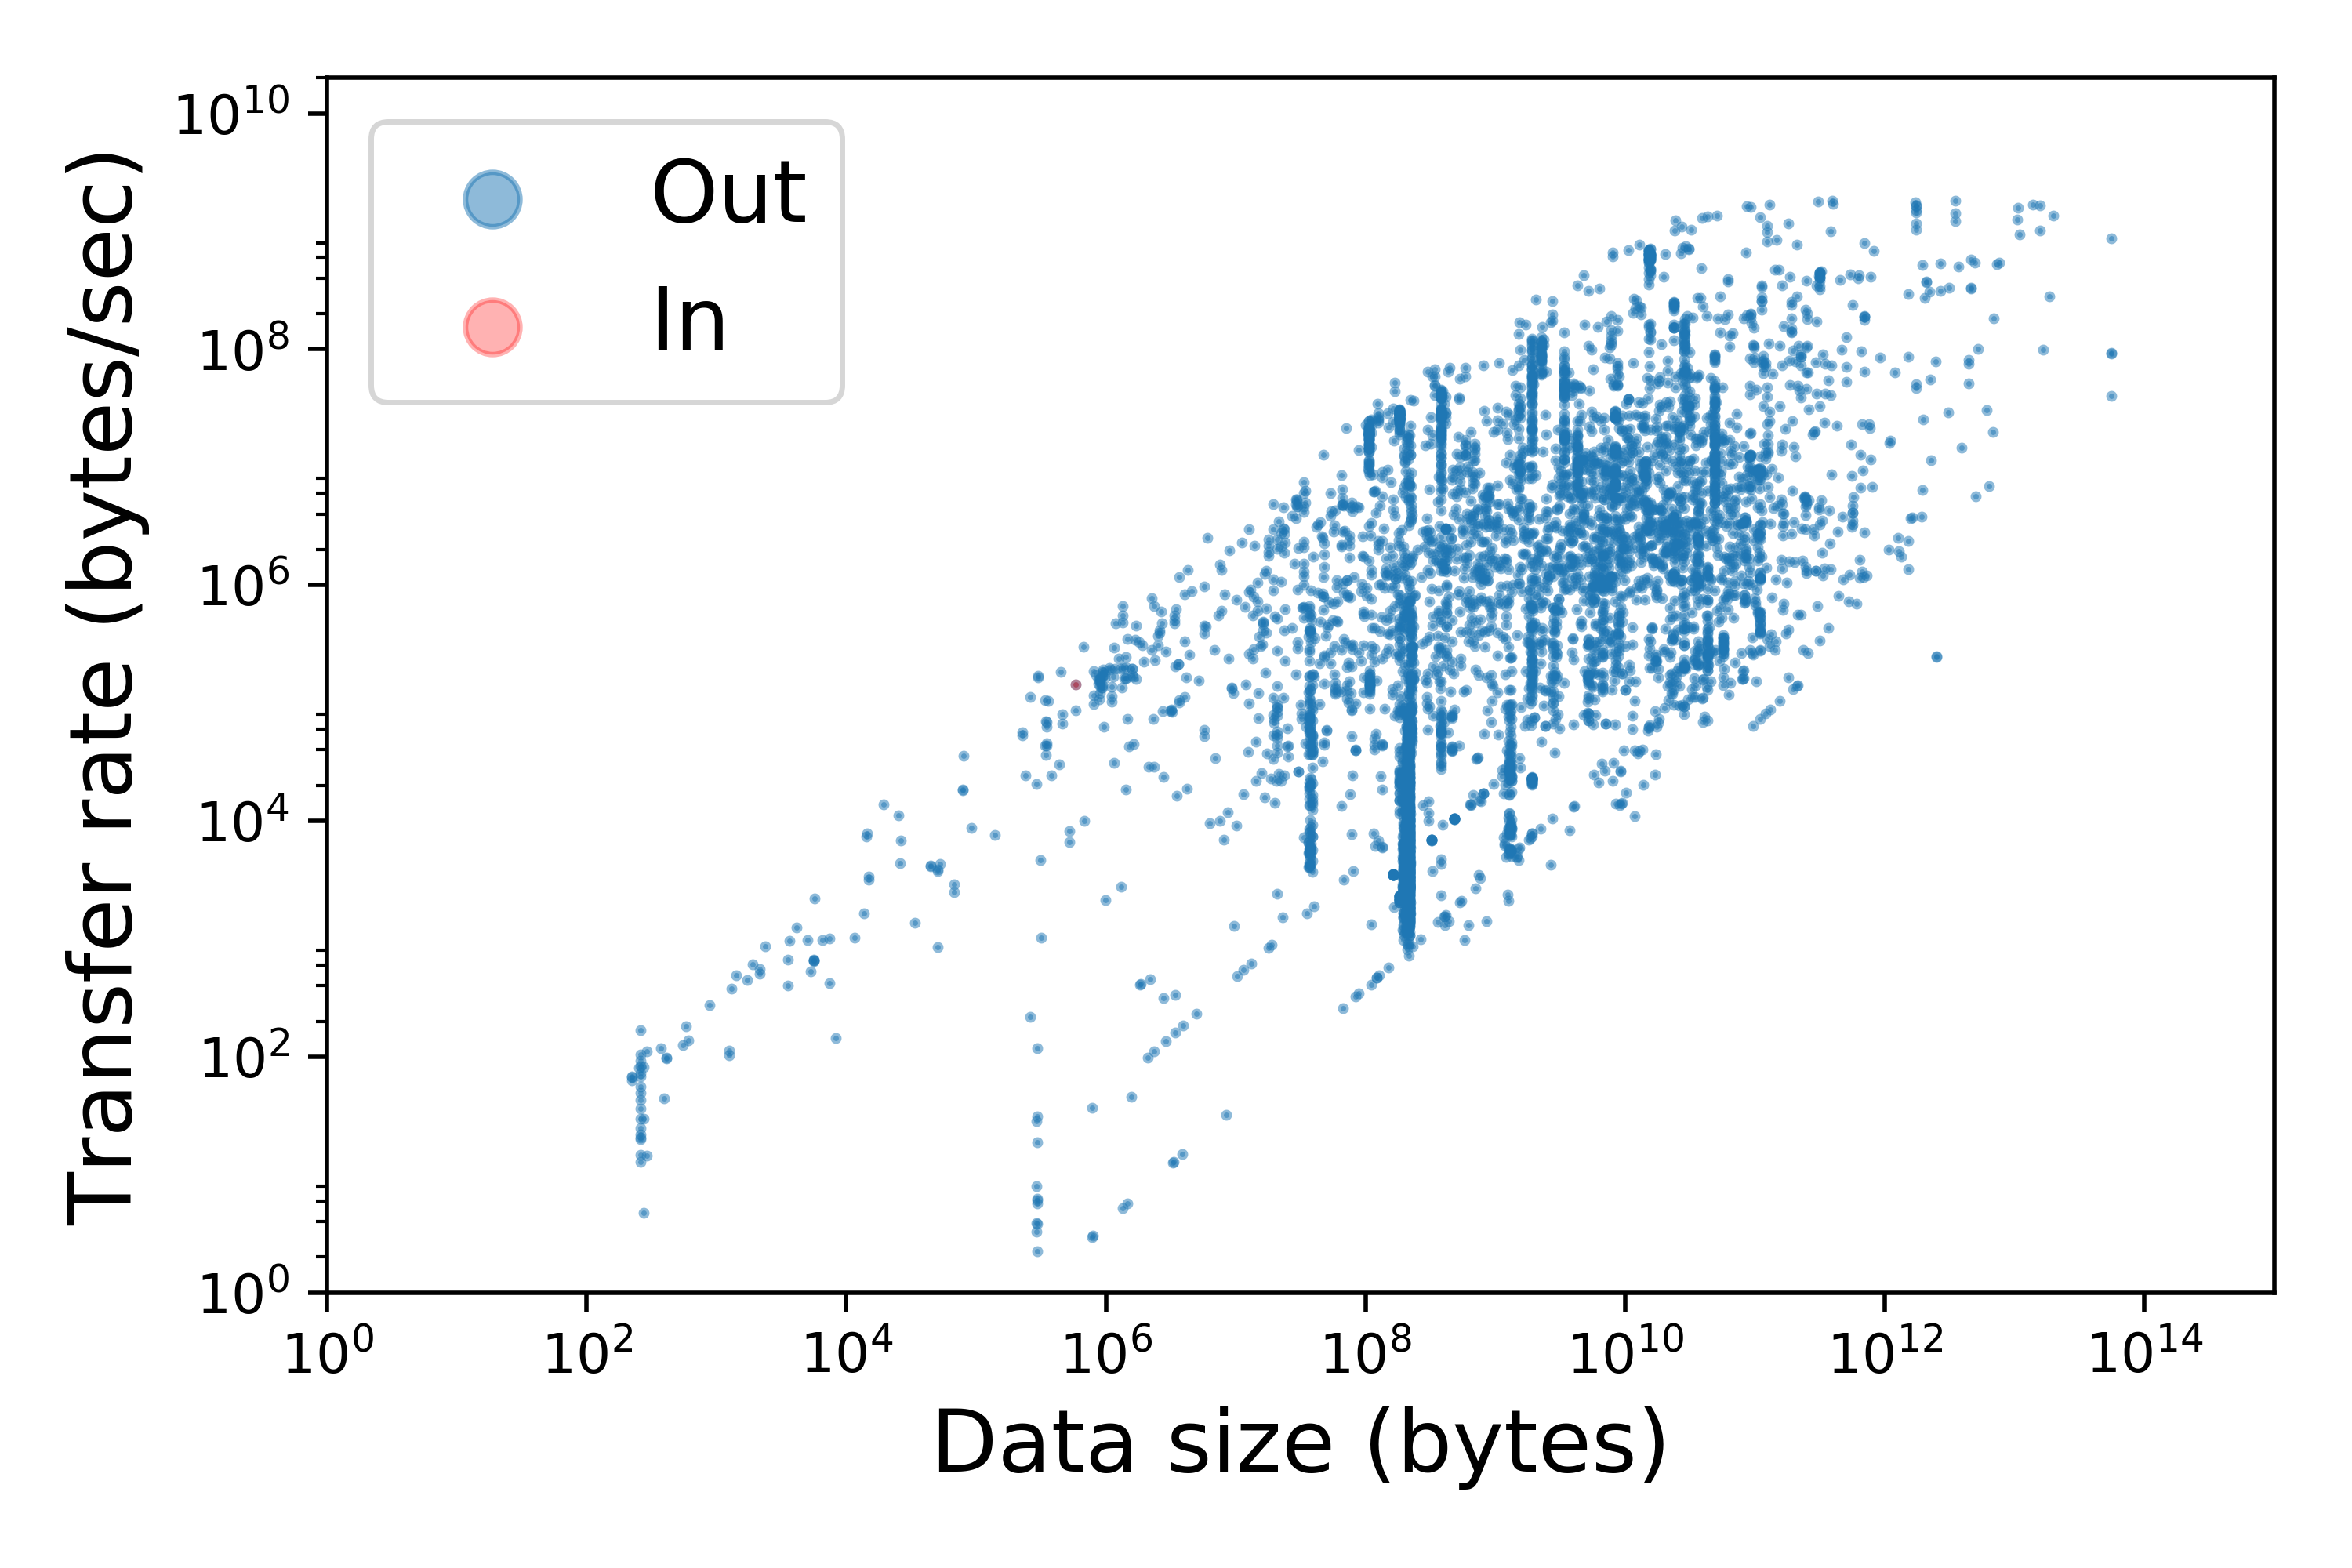
\includegraphics[width=0.47\textwidth,trim=0.14in 0.15in 0.15in 0.2in,clip]{Figures/rda-size-time.png} }
    \subfloat[RDA to NERSC subset]{\label{fig:rda-rate2}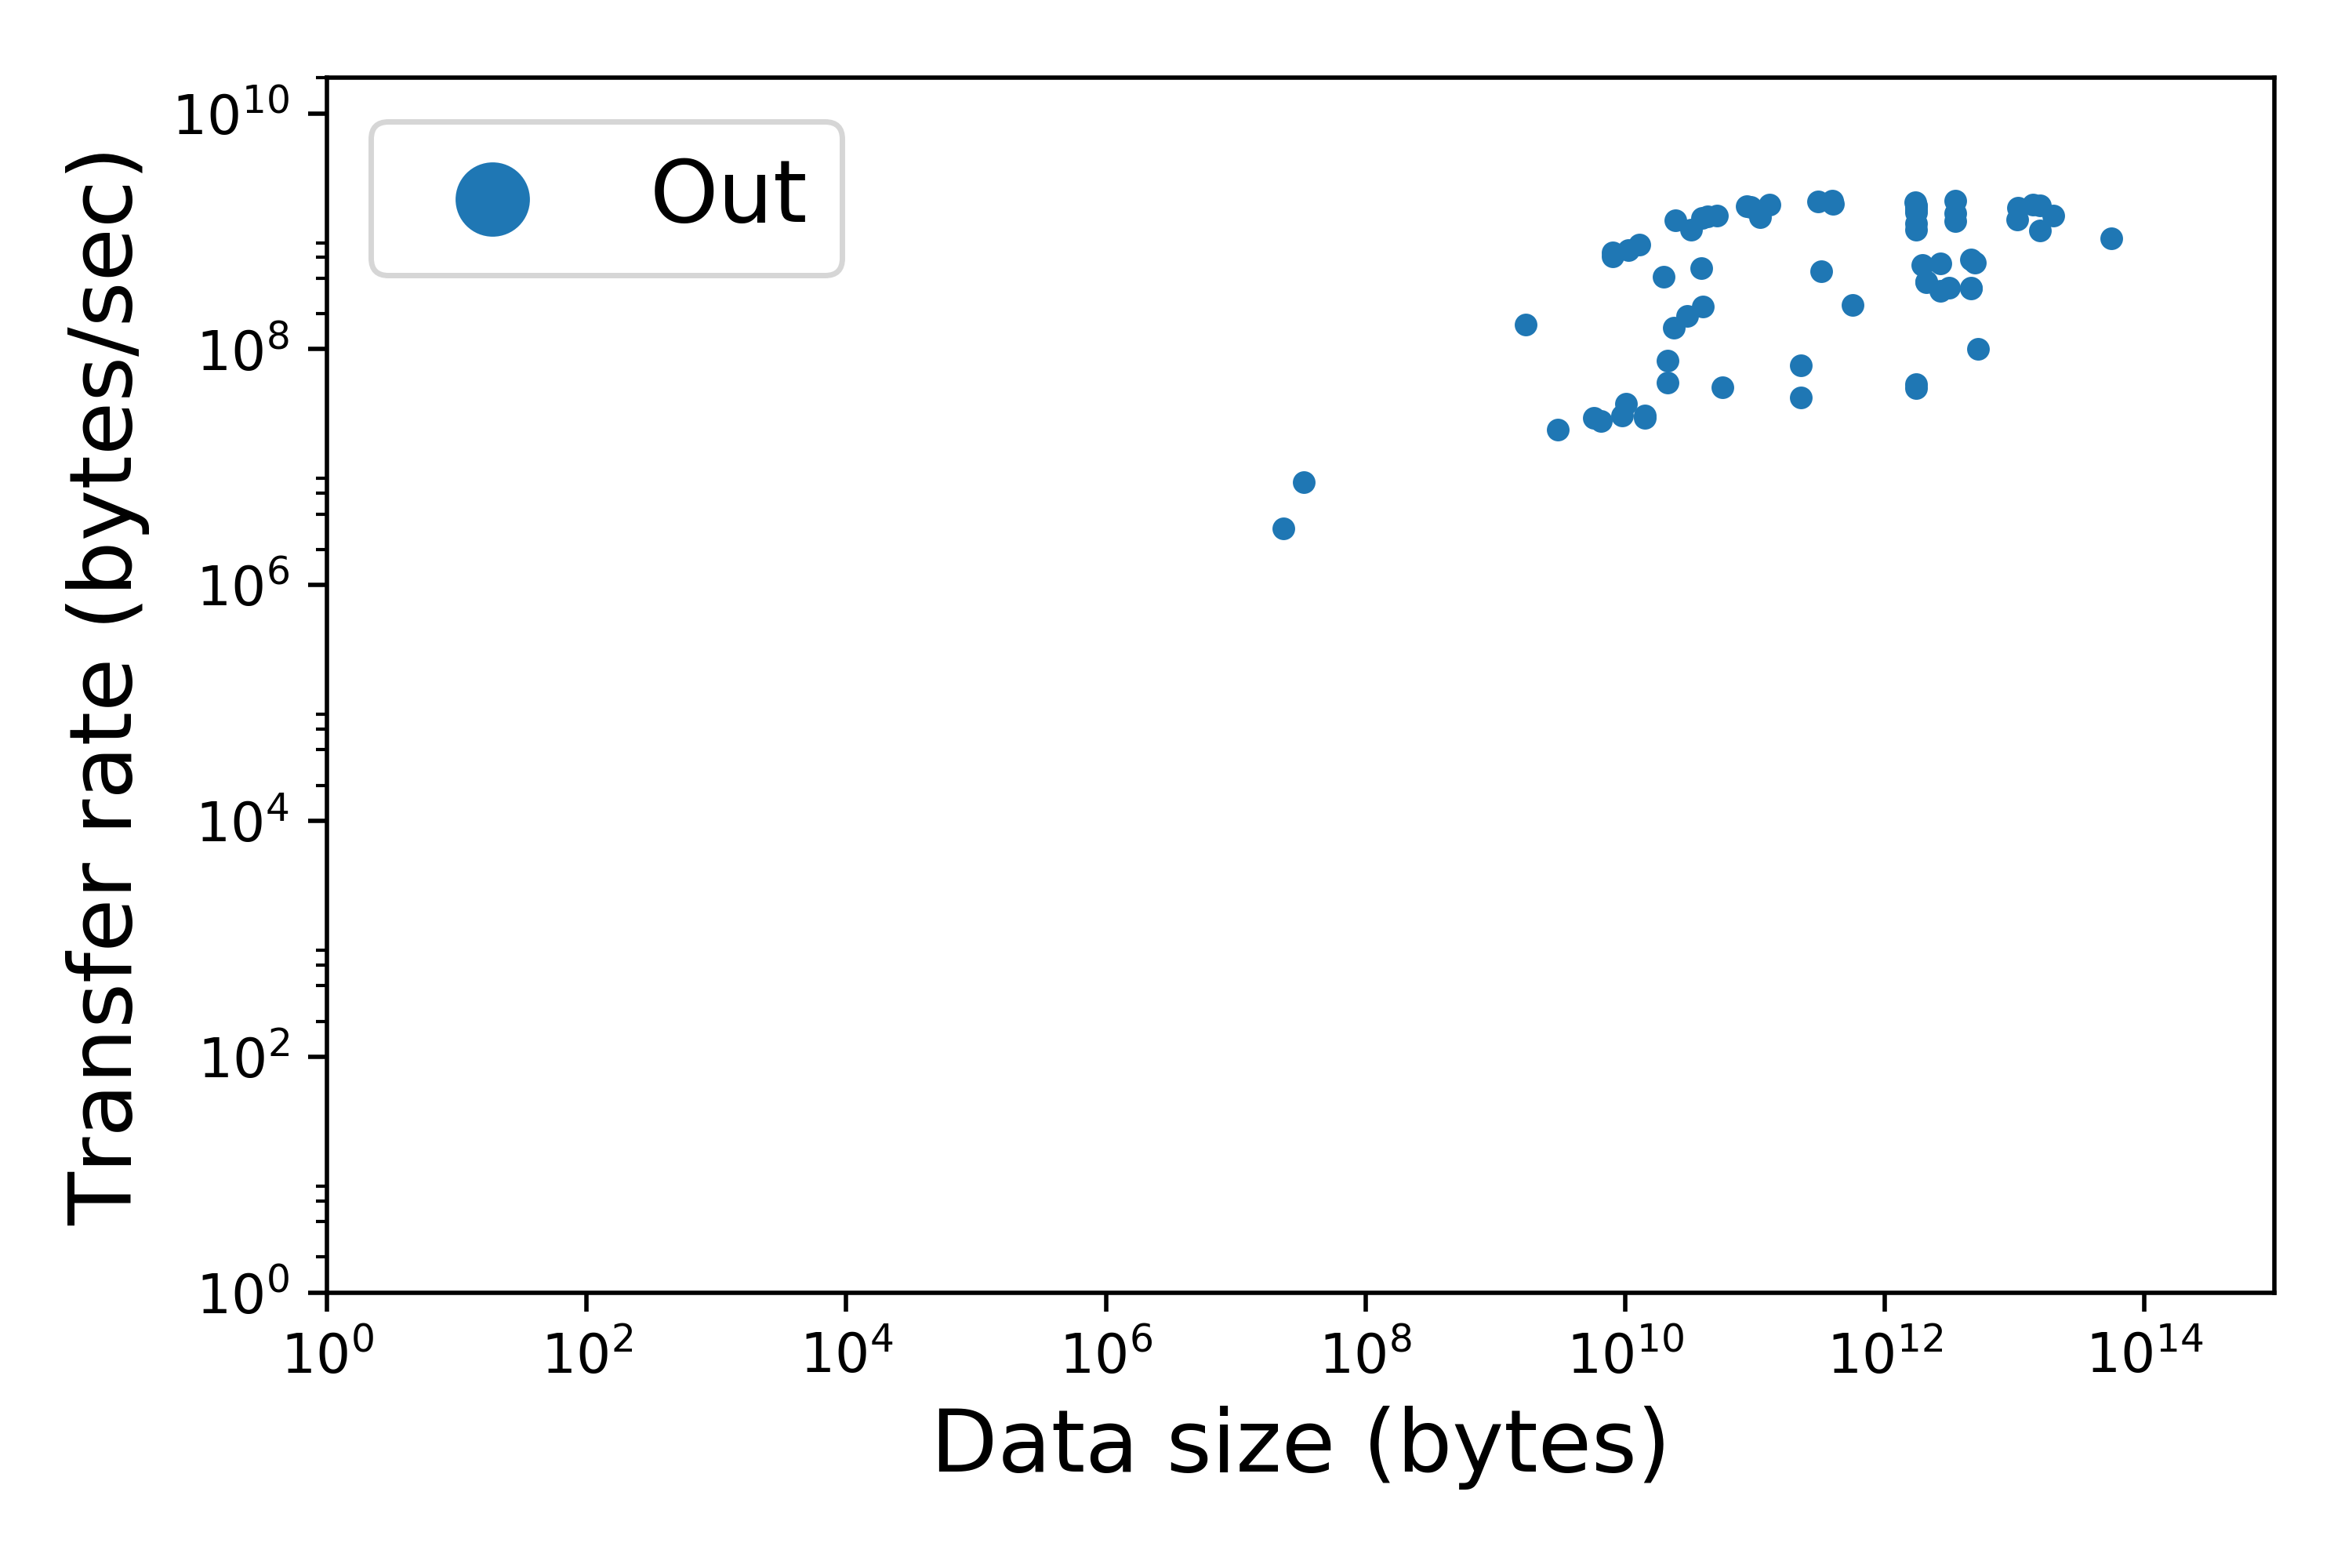
\includegraphics[width=0.47\textwidth,trim=0.14in 0.15in 0.15in 0.2in,clip]{Figures/nersc-size-time.png}}\\

  \vspace{1ex}
  
\caption{Transfer rate vs.\ data size for the RDA portal:
(a) all transfers and 
(b) only transfers from RDA to NERSC, with points 
in a larger size.
Each point represents a single transfer, which may involve many files.
Incoming and outgoing transfers are distinguished on the left, but
RDA has only one incoming transfer.
}
\label{fig:sizetime}
\end{figure}



\section*{Design pattern \#2: Automation for Research Facilities}

The second pattern is concerned with 
the automation of mundane but critical tasks that relate to the acquisition 
and dissemination of data from instruments, experimental facilities, and large-scale simulations.
Its implementation uses many of the constructs applied in the MRDP pattern, but for a different purpose. 

User facilities that host instruments face the challenge of providing automated secure data management workflows to their users enabling them to access data they have collected when they need it, where they need it and in formats needed by their processing tools. 
While data types and volumes, and duration of experiment may vary, instrument facilities ranging from campus core facilities that have sequencers or microscopes, to national facilities such as the light sources, have a common need for scalable secure data management solutions. 
With the facility operating around the clock, and beam time use as a key metric, operators of the facility need services and solutions that not only allows them to automate a large part of the data management workflow, but also provides them with a platform that can be extended and integrated with their local authentication and data flow systems.

Current practices often require copying of the collected data into physical media that is then carried back to the user's home institution for analysis and sharing. 
This process is error prone and time consuming, and furthermore does not provide any timely feedback to the experiment such that users can improve the quality of data gathered while they are at the facility. 
It also places the burden on the researchers to ensure integrity of the copied data, 
and significantly increases the time to results from such experiments.

% KC: what data management platform? is this what we are proposing? Or something that exists?
The scalable data management platform leverages the high performance network at institutions, 
science DMZ concepts and a platform for secure data sharing to deliver a solution that allows near-real time data access at high speeds, 
while still providing fine grained access control permissions on the data. 

Data access is via DTNs that are directly connected to high bandwidth networks to allow efficient data transfer to and from these nodes. 
Acquisition machines that gather data either share a file system with the DTNs or use automated internal transfers to move data to DTN-accessible storage.
(See \url{github.com/globus/automation-examples} for example code for such transfers.)
Security integration that leverages local authentication and policy is made possible by using Globus Auth, which allows single sign on with federated identity and secure access to data management services using standards such as OAuth 2.0. 
Data sharing services that leverage this security platform,
such as Globus Sharing,
provide fine-grained access control, 
allowing a facility to ensure that experiment data are available only to authorized users . 

This design pattern, like the first, makes heavy use of Globus platform APIs to integrate Globus security and data sharing features with existing facility data management workflows and user management system
This usage is critical to delivering an end-to-end solution that 
enables instant and automate data sharing. % and thus more rapid
%reduces the time to process and gather insights from the data 
%This dramatically changes the model from gathering data and using physical media to take data back to the user's institution at the end of the experiment to process, to instantly sharing the data for remote access. 



\subsection*{Automation case study: Light source data pipelines}

The Advanced Photon Source (APS) at Argonne National Laboratory is typical of many experimental facilities
worldwide in that it serves large numbers (thousands) of researchers every year,
most of whom visit just for a few days to collect data and then return to their home institution.
In the past, data produced during an experiment was invariably carried back on physical media.
However, as data sizes have grown and experiments have become more collaborative,
that approach has become less effective.
Users want to share data with remote collaborators during an experiment, 
for example for quality control.
Data transfer via network is needed;
the challenge is to integrate data transfer into the experimental workflow of the facility
in a way that is fully automated, secure, reliable, and scalable to thousands of users and datasets.

Several APS beamlines have adopted a solution that uses the research automation pattern to
leverage high performance DTNs
and to link local authentication and authorization to their experiment management system and Globus data services. 
DMagic (\url{dmagic.readthedocs.io}) provides the implementation.
When an experiment is approved,
a set of associated researchers are registered in the APS administrative database as approved participants.
Before the experiment begins,
DMagic creates a shared endpoint on an Argonne storage system with high-speed DTN access.
DMagic then retrieves from the APS scheduling system the list of approved users for the experiment,
and uses Globus APIs to grant those users read permissions on the shared endpoint.
%Globus support for roles allows the PIs of the experiment autonomy in managing further access to the data on the shared endpoint. 
It then monitors the experiment data directory at the APS facility and copies
new files automatically to that shared endpoint,
from which it can be retrieved by any approved user.
APS facility operators also have access to administrative and monitoring capabilities that allow them to check for successful transfer of the data prior to deleting data from their local storage.

%
%Using Globus Auth, the users get single sign-on using APS login, 
%and Globus sharing is used to set up secure sharing policies on the data collected for each experiment. 
%When an experiment is started, a shared endpoint is created with permissions from the APS experiment management system to allow the approved set of users to have read permissions on the endpoint. 
%This uses the DTNs and thus provides a fast, and efficient network for data flowing outside the institution, that Globus transfer leverages to provide reliable and performant data transfers. 


%\begin{wrapfigure}
%    \centering
%    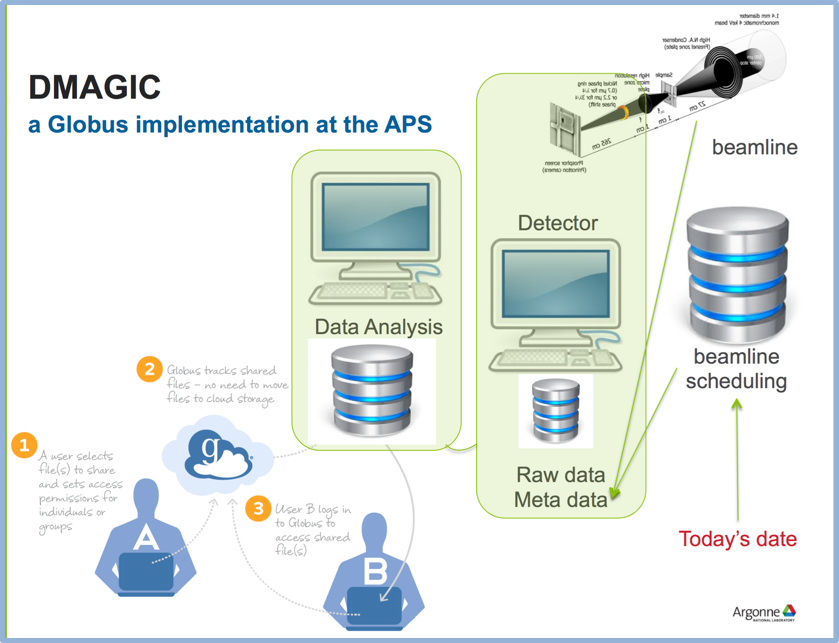
\includegraphics[trim=0 0 0 0,clip,width=0.8\columnwidth]{Figures/DMagic.png}
%    \caption{XXX
%    \label{fig:simple}}
%\end{wrapfigure}


\section*{Background on the Globus services used in the design patterns}
Globus provides data and identity management capabilities designed for the research community. 
These capabilities are delivered via a cloud-hosted software- and platform-as-a-service model, 
enabling users to access them through their web browser and
developers to invoke them via powerful APIs. 
We describe here Globus capabilities for managing and transferring data and for authenticating users and authorizing access.

Globus allows data to be remotely managed across its pool of more than 10,000 accessible storage systems (called ``endpoints''). 
A storage system is made accessible to Globus, and thus capable of high performance and reliable data transfer, by installing Globus Connect software. 
Globus Connect is offered in two versions: 
Globus Connect Personal for single-user deployments (e.g., a laptop or PC) and Globus Connect Server for multi-user
deployments (e.g., a shared server or DTN). 

Globus Transfer capabilities provide high performance and reliable third party data transfer. 
The Globus service manages the entire transfer process, including coordinating authentication at source and destination; establishing a high performance data channel using  the GridFTP protocol, with configuration optimized for transfer; ensuring data integrity by comparing source/destination checksums; and recovering from any errors during the transfer.  Globus, by default, enforces the data access permissions represented
by the underlying system; however, it also allows these access decisions to be managed through the cloud service. In the latter mode, called Globus Sharing, users may associate user- or group-based access control lists (ACLs) with particular file paths. Globus checks and enforces these ACLs when other users attempt to read or write to those paths.

Globus Auth provides identity and access management platform capabilities. It brokers authentication and authorization interactions between end-users, identity providers, resource servers (services), and clients (e.g., web, mobile, desktop, and command line applications, and other services). 
It implements standard web protocols, such as OAuth 2.0 and OpenID Connect, that allow it to be integrated easily with external applications using standard client libraries. 
These protocols enable third-party applications to authenticate users (using their preferred identity) directly with the chosen identity provider. Globus Auth then returns access
tokens that the third-party application can use to validate the user's identity and to perform actions on behalf of that user, within an agreed upon scope. Globus Auth implements an identity federation model via which diverse identities can be linked, and such that presentation of one identity may support authorization for the set of identities. Integration with Globus Groups supports group-based authorization using user-managed groups.

\section*{Summary}

We have presented two design patterns that capture important characteristics of 
data-driven discovery systems that we have observed in frequent use. 
Our goal in so doing is to reduce the costs associated with assisting research teams
by suggesting stylized ways of thinking about their problems and then describing
proven methods for addressing those problems.
We believe that, as in other areas of computing, 
the identification and use of familiar design patterns 
can simplify development, deployment, and operation.

% 

The two design patterns and three use cases that we present here
illustrate how existing infrastructure (e.g., storage and compute provided by a research computing center) can be enhanced via the use of higher level ``building blocks'' provided by the Globus platform, including authentication and authorization, data access and transfer, and data publication and discovery. 
Collectively, as these examples show, Globus capabilities address the entire data lifecycle: from data acquisition through to publication and archiving. 
The widespread deployment of Globus services makes it straightforward to extend
the reach of systems constructed with these patterns across campuses and institutions.


\section*{Acknowledgments}

We thanks the Globus team for the development of the technologies described here.
This work was supported in part by NSF grant ACI-1148484 and by the DOE under contract DE-AC02-06CH11357.

\small
\bibliographystyle{abbrv}
\bibliography{bib}

\end{document}
